\section{背景}
\label{sec:background}

\subsection{Agentic RL 训练}
\label{subsec:multi-task-agentic}

\PHB{训练流水线。}
多任务 agentic RL 的训练流程由三个计算阶段构成循环。首先是用于采样经验的 \textbf{rollout} 阶段：智能体 LLM 与多个并行环境交互，生成训练数据。与普通 LLM 推理不同，这一过程具备\emph{多轮}与\emph{有状态}特征~\cite{kimiteam2025kimik2openagentic,deepseek_v3_2_speciale}。在每一轮里，智能体观察状态、生成动作序列并提交给环境，环境执行动作后返回反馈，直到满足终止条件，形成由状态-动作对组成的\emph{轨迹}。随后进入 \textbf{reward} 阶段，奖励工作者对轨迹质量进行评估，从轻量级规则打分~\cite{he2025deepmath} 到基于模型的裁判式判断~\cite{son2024llmasajudgerewardmodel,zhong2024rlhfuseefficientrlhftraining} 都属于这一阶段。最后，\textbf{training} 阶段利用这些轨迹和奖励通过 PPO、GRPO 等算法更新参数~\cite{schulman2017proximal,shao2024deepseekmath}。出于训练性能考虑，很多 RL 系统仍然采用\emph{同步}范式，即要求 rollout 与 training 在每一步严格对齐模型权重~\cite{areal}。

\begin{table}[t]
\centering
\caption{本文采用的 agentic 环境分类。}
\label{tab:env-taxomy}
\resizebox{0.48\textwidth}{!}{%
\begin{tabular}{ll l c}
\toprule
\textbf{环境} & \textbf{任务领域} & \textbf{模态} & \textbf{轮次数} \\
\midrule
SWE-bench~\cite{swe-bench} & 软件工程 & 文本 & 30--50 \\
WebShop~\cite{webshop} & Web & 文本 & 5--30 \\
FrozenLake~\cite{frozen_lake} & 游戏 & 文本、视觉 & 20--100 \\
GEM-math~\cite{GEM-github} & 数学+工具调用 & 文本 & $<5$ \\
GEM-game~\cite{GEM-github} & 游戏 & 文本 & 1 \\
\bottomrule
\end{tabular}}
\end{table}

\begin{figure}[tb]
\centering
\begin{subfigure}{0.48\textwidth}
\centering
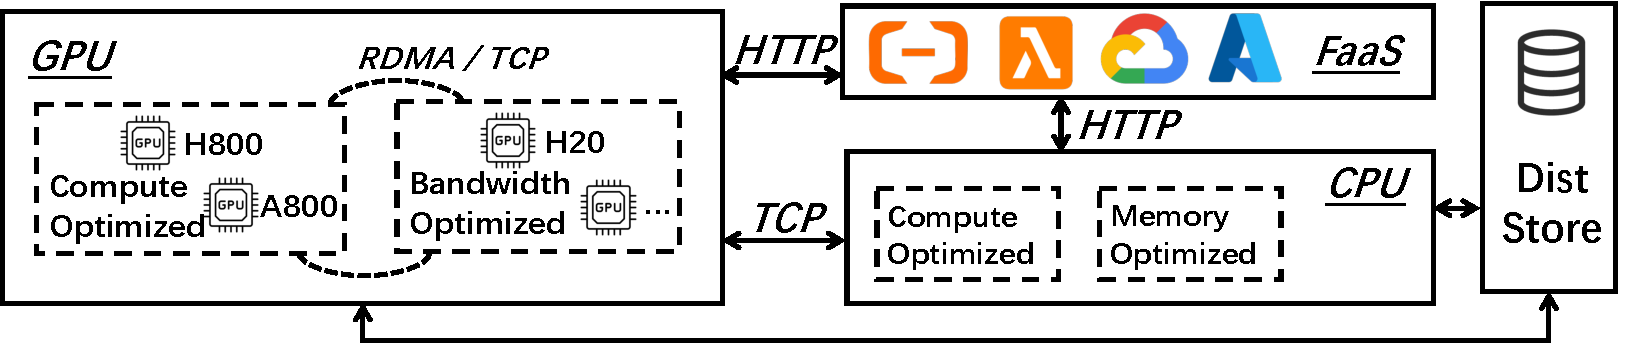
\includegraphics[width=\linewidth]{figs/overview/disaggregated_cluster.pdf}
\end{subfigure}
\caption{面向 agentic RL 训练的解耦式基础设施。}
\label{fig:disaggregated_cluster}
\end{figure}

\PHM{环境异构性。}
agentic RL 的一个关键挑战是环境极其多样，而这种多样性直接决定了系统计算画像。\autoref{tab:env-taxomy} 显示，不同任务在模态、交互轮次以及环境复杂度上差异极大。长回合任务需要频繁维护上下文与环境状态，往往由 prefill 代价主导；而短回合任务更多体现为高频 decoding。环境本身还可能依赖浏览器、Docker、代码沙箱、数据库或外部网络服务，因此其瓶颈可能来自 CPU、磁盘、网络或容器生命周期管理，而非 GPU。

\PHB{为何需要解耦。}
这种异构性决定了“一个资源池包打天下”的方式效率很低。理想情况下，训练应运行在高算力 GPU 上，环境应运行在 CPU 集群上，奖励模型则可以部署在独立 GPU 或 serverless 平台中。更进一步，在 rollout 内部，不同任务也应被分配到不同 GPU。例如 prefill 主导任务更适合 H800，而 decode 主导任务可能更适合 H20。如果所有 rollout 都绑定到同一种 GPU，系统将难以充分利用可用硬件。

\PHM{同步训练与异步训练。}
同步 RL 训练实现简单，也有利于控制样本新鲜度，但在 agentic RL 中代价很高。环境的长尾延迟、失败重试、不同任务的轮次差异都会让整批样本被最慢的少数轨迹拖住。异步训练允许 rollout 与 training 并行推进，训练端可以在一定范围内消费略旧的样本，以换取更高吞吐。但异步也引入样本陈旧性与稳定性风险，因此需要一套精细的控制机制来限制旧轨迹被使用的程度。

\PHB{单步训练延迟拆解。}
我们在 \texttt{SWE-bench} 上分析一步训练的耗时。环境初始化主要由 Docker 镜像拉取、容器启动和沙箱准备构成；环境执行则受代码运行和交互逻辑影响；LLM 生成主导大部分 GPU 时间。实验显示，在完全成功的迭代里，生成阶段是主要开销；但在包含环境失败的迭代里，\texttt{env.reset} 会迅速成为瓶颈，平均步时从约 366 秒增加到 513 秒，其中仅环境初始化就可占 rollout 时间的 78\%。这说明在 agentic RL 中，环境生命周期管理不是边缘问题，而是核心系统问题。

\begin{figure}[t]
\centering
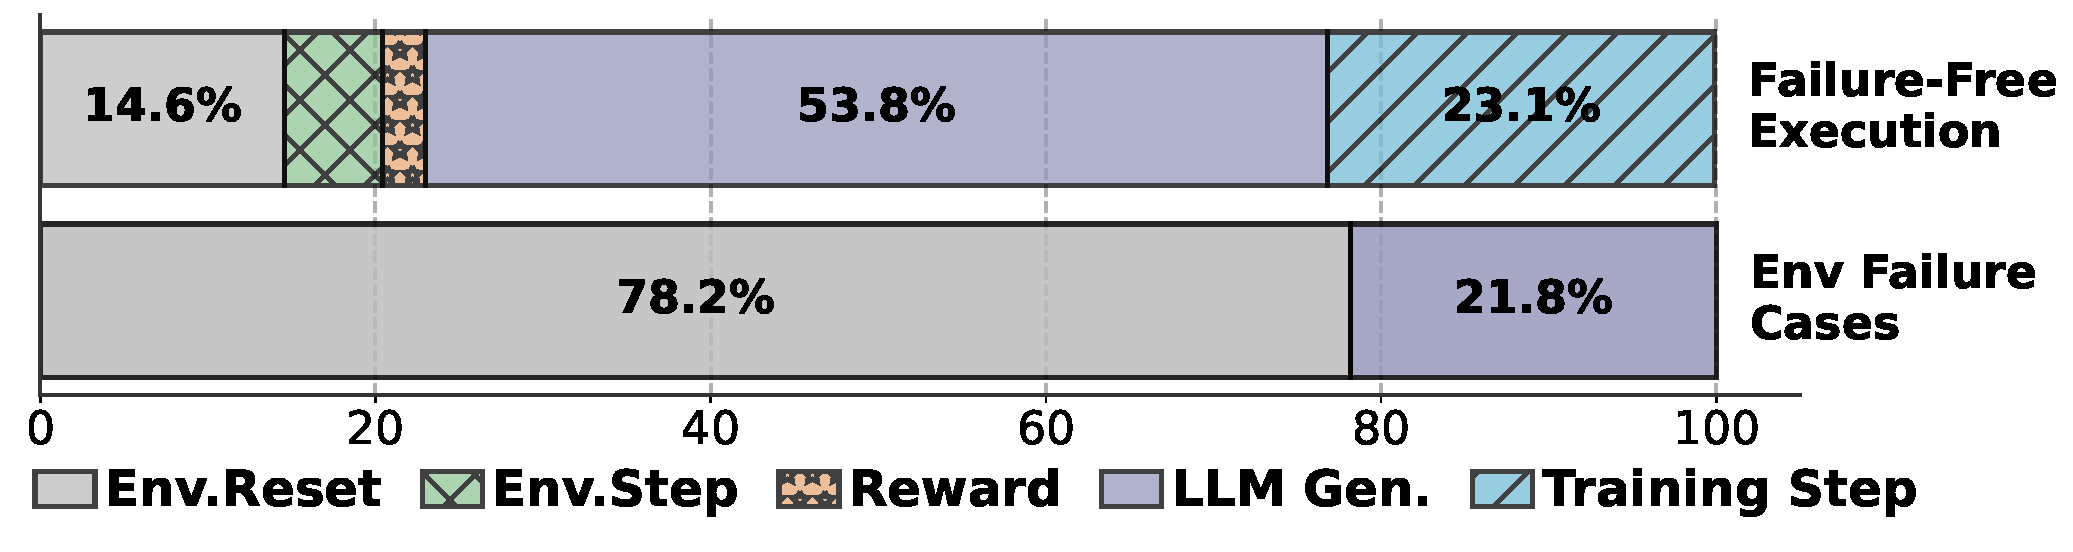
\includegraphics[width=\linewidth]{figs/time/Qwen3-8B-GPU16-sync_time_distribution_fixed.pdf}
\caption{训练步耗时分解：上图为成功执行， 下图为伴随环境失败的执行。}
\label{fig:time_breakdown}
\end{figure}

\begin{figure}[tb]
\centering
\begin{subfigure}{0.235\textwidth}
\centering
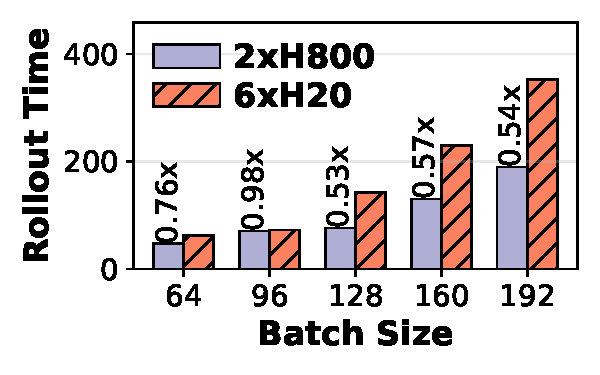
\includegraphics[width=\linewidth]{figs/disagg_motivation/osdi_frozen_lake_decoding_1024_bar.pdf}
\caption{\texttt{FrozenLake}（prefill 主导）。}
\label{fig:prefill-heavy-task}
\end{subfigure}
\begin{subfigure}{0.235\textwidth}
\centering
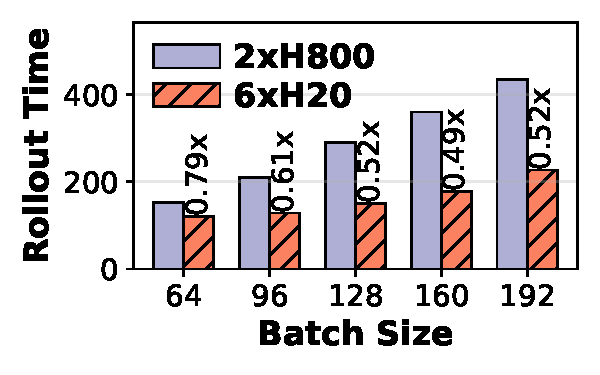
\includegraphics[width=\linewidth]{figs/disagg_motivation/osdi_gem_math_thinking_decoding_4096_bar.pdf}
\caption{\texttt{GEM-Math}（decoding 主导）。}
\label{fig:decode-heavy-task}
\end{subfigure}
\caption{在 H20 与 H800 上，不同任务随 batch size 变化的 rollout 总时长。}
\label{fig:motivation-task-affinity}
\end{figure}

\PHM{生成阶段存在分化的硬件亲和性。}
现代 GPU 在算力、显存容量、带宽与成本上存在不同权衡。已有工作倡导将 rollout 与 training 分置到不同 GPU 上~\cite{StreamRL,asyncflow,seamlessflow}，但我们的测量表明，\emph{对 agentic 工作负载而言，这种静态划分仍不够细}。LLM 生成同时包含 prefill 与 decoding 两个资源特征完全不同的阶段；同一个 rollout 集群里，不同任务可能对不同 GPU 呈现截然不同的偏好。\autoref{fig:motivation-task-affinity} 就显示，\texttt{FrozenLake} 更适合算力型设备，而 \texttt{GEM-Math} 在带宽型设备上更高效。

\PHB{长尾环境执行。}
真实环境存在明显长尾分布。浏览器环境可能因页面加载而阻塞，代码环境可能因容器初始化失败而超时，游戏环境则可能出现异常重置。若系统坚持批次同步，就必须等待最慢环境完成，从而把大量 GPU 时间浪费在空转上。更合理的方式是按轨迹管理环境状态，让慢环境不阻塞快环境，并允许系统主动终止那些超出容忍窗口的执行。

\PHB{无状态奖励计算。}
奖励计算通常只依赖输入轨迹，不依赖历史状态，这使其天然适合 serverless 平台：按需启动、自动扩缩容、多租户共享、失败隔离都更容易实现。与其为奖励模型常驻预留 GPU，不如把它变成一种共享式的 Reward-as-a-Service。

\PHB{稳定性优先的轨迹传输。}
轨迹数据本身相对权重同步来说并不大，但它出现在高频环境交互路径中。因此，轨迹传输更强调网络稳定性和低抖动，而不只是峰值带宽。通过把环境交互与 LLM 生成异步化，系统可以隐藏网络波动带来的停顿。

\PHM{带宽密集的权重更新。}
与轨迹不同，模型权重同步是真正的带宽密集型通信。它需要高吞吐传输引擎与跨集群优化，否则会吞噬异步训练带来的收益。这一观察意味着系统必须为不同类型的数据流使用不同的传输策略，而不是统一采用同一套通信机制。
